\documentclass[openany]{book}
\usepackage{lmodern}
\usepackage{amssymb,amsmath}
\usepackage{ifxetex,ifluatex}
\usepackage{fixltx2e} % provides \textsubscript
\ifnum 0\ifxetex 1\fi\ifluatex 1\fi=0 % if pdftex
  \usepackage[T1]{fontenc}
  \usepackage[utf8]{inputenc}
\else % if luatex or xelatex
  \ifxetex
    \usepackage{mathspec}
  \else
    \usepackage{fontspec}
  \fi
  \defaultfontfeatures{Ligatures=TeX,Scale=MatchLowercase}
\fi
% use upquote if available, for straight quotes in verbatim environments
\IfFileExists{upquote.sty}{\usepackage{upquote}}{}
% use microtype if available
\IfFileExists{microtype.sty}{%
\usepackage{microtype}
\UseMicrotypeSet[protrusion]{basicmath} % disable protrusion for tt fonts
}{}
\usepackage[margin=1in]{geometry}
\usepackage{hyperref}
\hypersetup{unicode=true,
            pdftitle={DATA 624: Project 1},
            pdfauthor={Bethany Poulin},
            pdfborder={0 0 0},
            breaklinks=true}
\urlstyle{same}  % don't use monospace font for urls
\usepackage{natbib}
\bibliographystyle{plainnat}
\usepackage{color}
\usepackage{fancyvrb}
\newcommand{\VerbBar}{|}
\newcommand{\VERB}{\Verb[commandchars=\\\{\}]}
\DefineVerbatimEnvironment{Highlighting}{Verbatim}{commandchars=\\\{\}}
% Add ',fontsize=\small' for more characters per line
\usepackage{framed}
\definecolor{shadecolor}{RGB}{248,248,248}
\newenvironment{Shaded}{\begin{snugshade}}{\end{snugshade}}
\newcommand{\AlertTok}[1]{\textcolor[rgb]{0.94,0.16,0.16}{#1}}
\newcommand{\AnnotationTok}[1]{\textcolor[rgb]{0.56,0.35,0.01}{\textbf{\textit{#1}}}}
\newcommand{\AttributeTok}[1]{\textcolor[rgb]{0.77,0.63,0.00}{#1}}
\newcommand{\BaseNTok}[1]{\textcolor[rgb]{0.00,0.00,0.81}{#1}}
\newcommand{\BuiltInTok}[1]{#1}
\newcommand{\CharTok}[1]{\textcolor[rgb]{0.31,0.60,0.02}{#1}}
\newcommand{\CommentTok}[1]{\textcolor[rgb]{0.56,0.35,0.01}{\textit{#1}}}
\newcommand{\CommentVarTok}[1]{\textcolor[rgb]{0.56,0.35,0.01}{\textbf{\textit{#1}}}}
\newcommand{\ConstantTok}[1]{\textcolor[rgb]{0.00,0.00,0.00}{#1}}
\newcommand{\ControlFlowTok}[1]{\textcolor[rgb]{0.13,0.29,0.53}{\textbf{#1}}}
\newcommand{\DataTypeTok}[1]{\textcolor[rgb]{0.13,0.29,0.53}{#1}}
\newcommand{\DecValTok}[1]{\textcolor[rgb]{0.00,0.00,0.81}{#1}}
\newcommand{\DocumentationTok}[1]{\textcolor[rgb]{0.56,0.35,0.01}{\textbf{\textit{#1}}}}
\newcommand{\ErrorTok}[1]{\textcolor[rgb]{0.64,0.00,0.00}{\textbf{#1}}}
\newcommand{\ExtensionTok}[1]{#1}
\newcommand{\FloatTok}[1]{\textcolor[rgb]{0.00,0.00,0.81}{#1}}
\newcommand{\FunctionTok}[1]{\textcolor[rgb]{0.00,0.00,0.00}{#1}}
\newcommand{\ImportTok}[1]{#1}
\newcommand{\InformationTok}[1]{\textcolor[rgb]{0.56,0.35,0.01}{\textbf{\textit{#1}}}}
\newcommand{\KeywordTok}[1]{\textcolor[rgb]{0.13,0.29,0.53}{\textbf{#1}}}
\newcommand{\NormalTok}[1]{#1}
\newcommand{\OperatorTok}[1]{\textcolor[rgb]{0.81,0.36,0.00}{\textbf{#1}}}
\newcommand{\OtherTok}[1]{\textcolor[rgb]{0.56,0.35,0.01}{#1}}
\newcommand{\PreprocessorTok}[1]{\textcolor[rgb]{0.56,0.35,0.01}{\textit{#1}}}
\newcommand{\RegionMarkerTok}[1]{#1}
\newcommand{\SpecialCharTok}[1]{\textcolor[rgb]{0.00,0.00,0.00}{#1}}
\newcommand{\SpecialStringTok}[1]{\textcolor[rgb]{0.31,0.60,0.02}{#1}}
\newcommand{\StringTok}[1]{\textcolor[rgb]{0.31,0.60,0.02}{#1}}
\newcommand{\VariableTok}[1]{\textcolor[rgb]{0.00,0.00,0.00}{#1}}
\newcommand{\VerbatimStringTok}[1]{\textcolor[rgb]{0.31,0.60,0.02}{#1}}
\newcommand{\WarningTok}[1]{\textcolor[rgb]{0.56,0.35,0.01}{\textbf{\textit{#1}}}}
\usepackage{graphicx,grffile}
\makeatletter
\def\maxwidth{\ifdim\Gin@nat@width>\linewidth\linewidth\else\Gin@nat@width\fi}
\def\maxheight{\ifdim\Gin@nat@height>\textheight\textheight\else\Gin@nat@height\fi}
\makeatother
% Scale images if necessary, so that they will not overflow the page
% margins by default, and it is still possible to overwrite the defaults
% using explicit options in \includegraphics[width, height, ...]{}
\setkeys{Gin}{width=\maxwidth,height=\maxheight,keepaspectratio}
\IfFileExists{parskip.sty}{%
\usepackage{parskip}
}{% else
\setlength{\parindent}{0pt}
\setlength{\parskip}{6pt plus 2pt minus 1pt}
}
\setlength{\emergencystretch}{3em}  % prevent overfull lines
\providecommand{\tightlist}{%
  \setlength{\itemsep}{0pt}\setlength{\parskip}{0pt}}
\setcounter{secnumdepth}{5}

%%% Use protect on footnotes to avoid problems with footnotes in titles
\let\rmarkdownfootnote\footnote%
\def\footnote{\protect\rmarkdownfootnote}

%%% Change title format to be more compact
\usepackage{titling}

% Create subtitle command for use in maketitle
\providecommand{\subtitle}[1]{
  \posttitle{
    \begin{center}\large#1\end{center}
    }
}

\setlength{\droptitle}{-2em}

  \title{DATA 624: Project 1}
    \pretitle{\vspace{\droptitle}\centering\huge}
  \posttitle{\par}
    \author{Bethany Poulin}
    \preauthor{\centering\large\emph}
  \postauthor{\par}
      \predate{\centering\large\emph}
  \postdate{\par}
    \date{October 22, 2019}

\usepackage{booktabs}
\usepackage[table]{xcolor}

% set plain style for page numbers
\pagestyle{plain}
\raggedbottom

% change font
\usepackage{fontspec}
\setmainfont{Arial}

% remove "chapter" from chapter title
\usepackage{titlesec}
\titleformat{\chapter}
  {\normalfont\LARGE\bfseries}{\thechapter}{1em}{}
\titlespacing*{\chapter}{0pt}{3.5ex plus 1ex minus .2ex}{2.3ex plus .2ex}

% create color block quotes
\usepackage{tcolorbox}
\newtcolorbox{myquote}{colback=orange!05!white, colframe=black!75!black}
\renewenvironment{quote}{\begin{myquote}}{\end{myquote}}

% wrap text
\usepackage{geometry}[textwidth=6in]

% kable 
\usepackage{tabu}
\usepackage{float}
\usepackage{booktabs}
\usepackage{longtable}
\usepackage{array}
\usepackage{multirow}
\usepackage{wrapfig}
\usepackage{float}
\usepackage{colortbl}
\usepackage{pdflscape}
\usepackage{tabu}
\usepackage{threeparttable}
\usepackage{threeparttablex}
\usepackage[normalem]{ulem}
\usepackage{makecell}
\usepackage{xcolor}

\begin{document}
\maketitle

{
\setcounter{tocdepth}{1}
\tableofcontents
}
\hypertarget{overview}{%
\chapter*{Overview}\label{overview}}
\addcontentsline{toc}{chapter}{Overview}

\begin{quote}
I am leaving the project overview page here for us to compile our final
report in one singular document. We will add additional information here
regarding project one to include explanation of process, etc.
\end{quote}

\hypertarget{dependencies}{%
\section*{Dependencies}\label{dependencies}}
\addcontentsline{toc}{section}{Dependencies}

\begin{quote}
Please add all libraries used here.
\end{quote}

The following R libraries were used to complete Project 1:

\begin{Shaded}
\begin{Highlighting}[]
\CommentTok{# General}
\KeywordTok{library}\NormalTok{(}\StringTok{'easypackages'}\NormalTok{)}

\KeywordTok{libraries}\NormalTok{(}\StringTok{'knitr'}\NormalTok{, }\StringTok{'kableExtra'}\NormalTok{, }\StringTok{'default'}\NormalTok{)}

\CommentTok{# Processing}
\KeywordTok{libraries}\NormalTok{(}\StringTok{'readxl'}\NormalTok{, }\StringTok{'tidyverse'}\NormalTok{, }\StringTok{'janitor'}\NormalTok{, }\StringTok{'lubridate'}\NormalTok{)}

\CommentTok{# Graphing}
\KeywordTok{libraries}\NormalTok{(}\StringTok{'ggplot2'}\NormalTok{, }\StringTok{'grid'}\NormalTok{, }\StringTok{'gridExtra'}\NormalTok{, }\StringTok{'ggfortify'}\NormalTok{,}\StringTok{'ggpubr'}\NormalTok{)}

\CommentTok{# Timeseries }
\KeywordTok{libraries}\NormalTok{(}\StringTok{'zoo'}\NormalTok{, }\StringTok{'urca'}\NormalTok{, }\StringTok{'tseries'}\NormalTok{, }\StringTok{'timetk'}\NormalTok{)}

\CommentTok{# Math}
\KeywordTok{libraries}\NormalTok{(}\StringTok{'forecast'}\NormalTok{)}
\end{Highlighting}
\end{Shaded}

\newpage

\hypertarget{data}{%
\section*{Data}\label{data}}
\addcontentsline{toc}{section}{Data}

Data was stored within our group repository and imported below using the
\texttt{readxl} package. Each individual question was solved within an R
script and the data was sourced into our main report for discussion
purposes. The R scripts are available within our appendix for
replication purposes.

For grading purposes, we exported and saved all forecasts as a csv in
our data folder.

\begin{Shaded}
\begin{Highlighting}[]
\CommentTok{# Data Aquisition}
\NormalTok{waterflow_}\DecValTok{1}\NormalTok{ <-}\StringTok{ }\KeywordTok{read_excel}\NormalTok{(}\StringTok{"data/Waterflow_Pipe1.xlsx"}\NormalTok{)}
\NormalTok{waterflow_}\DecValTok{2}\NormalTok{ <-}\StringTok{ }\KeywordTok{read_excel}\NormalTok{(}\StringTok{"data/Waterflow_Pipe2.xlsx"}\NormalTok{)}

\CommentTok{# Source Code}
\KeywordTok{source}\NormalTok{(}\StringTok{"scripts/Part-C-BP.R"}\NormalTok{)}
\end{Highlighting}
\end{Shaded}

\hypertarget{part-c}{%
\chapter{Part C}\label{part-c}}

\begin{quote}
Part C.consists of two data sets. These are simple 2 columns sets,
however they have different time stamps. Your assignment is to time-base
sequence the data and aggregate based on hour (example of what this
looks like, follows). Note for multiple recordings within an hour, take
the mean. Then to test appropriate assumptions and forecast a week
forward with confidence bands (80 and 95\%). Add these to your existing
files above – clearly labeled.
\end{quote}

\hypertarget{exploration}{%
\section{Exploration}\label{exploration}}

\textbf{Pipe one:}\\
* 1000 observations\\
* No missing values\\
* Multiple reading within each hour\\
* 9-days of data

\textbf{Pipe Two}\\
* 100 Observations\\
* No missing values\\
* Single reading on the hour\\
* 41-days of data

Because of the disparities in the data some grooming was necessary.\\
For Pipe One, representing 9-days of water flow rate measurements
multiple samples per hour, a mean of all rates in the hour was taken and
labeled with the whole-hour at the beggining of the period (floor hour)
to align with the hourly readings from Pipe Two.

After aggregating, there were only 236 observations (spanning 9-days) of
pipe one and still 1000 observations (spanning 41-days) from Pipe Two.

These data posed an interesting conundrum. With two possible ways of
handling it.\\
- Merge the files, and use only 236 observations\\
- all forecasts would be based on the combined data\\
- this would mean making 168 forecasts with only 236 data-points prior\\
- all forecasts would be starting November 1, instead of from the end of
data December 3\\
- Merge the files and use the whole set to make predictions\\
- we would have 100 observations to model prior to forecasts\\
- 236 of the observations would be be different from the remaining 764,
which could both alter the model type and forecast\\
- we would be forecasting from the natural ending of tPipe Two readings

Because it was concievable that there might be a daily periodicity, it
was important to have a frequency of 24, which made numbering by day of
year and grooming the time series to start on the 7081 hour aligning
with October 23 01:00 AM.

\hypertarget{time-series-plots}{%
\subsection{Time Series Plots}\label{time-series-plots}}

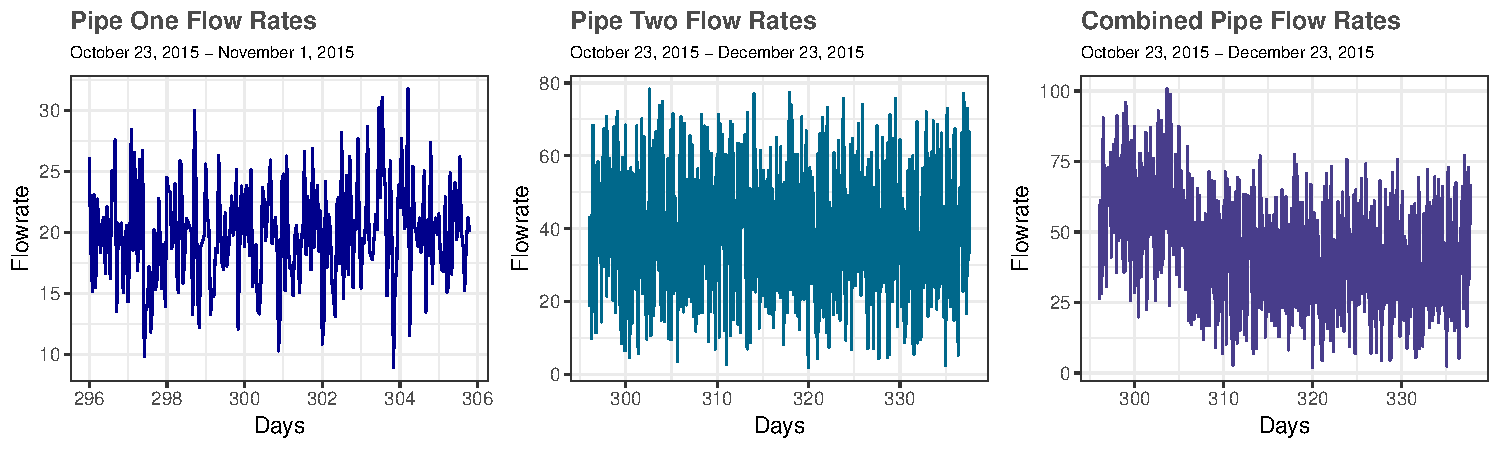
\includegraphics{Part-C-BP_files/figure-latex/unnamed-chunk-2-1.pdf}

\hypertarget{decomposition}{%
\subsection{Decomposition}\label{decomposition}}

It is clear from the combined plot that there is a pretty notable change
in the trend when the readings from Pipe One wane. Let's look at the
decomposed seriesand see if it gives us some insight into a good model.

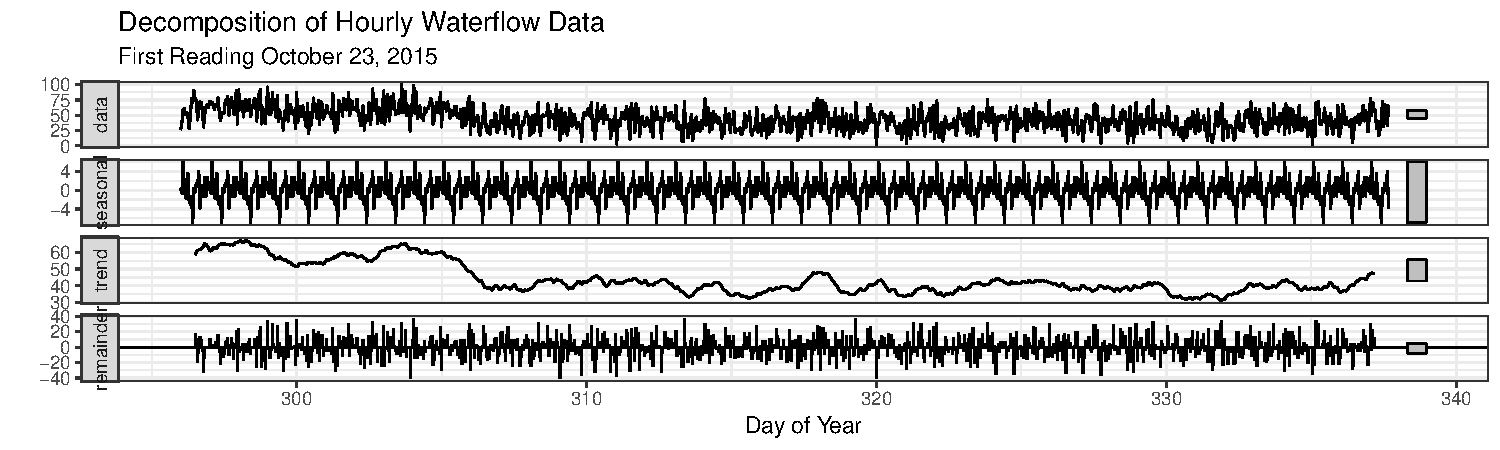
\includegraphics{Part-C-BP_files/figure-latex/unnamed-chunk-3-1.pdf}

From the decomposition, the appears to be a seasonal component in
agreement with the assessment that there might be a daily flowrate
periodicity. Also, as expected, around day 306 where Pipe One flow rates
go silent there is a trend down and then relatively flat trend
thereafter.

\hypertarget{estimating-stationarity}{%
\section{Estimating Stationarity}\label{estimating-stationarity}}

Number of Estimated Differences: 1

\begin{verbatim}
FALSE 
FALSE   Augmented Dickey-Fuller Test
FALSE 
FALSE data:  ws
FALSE Dickey-Fuller = -6.4409, Lag order = 9, p-value = 0.01
FALSE alternative hypothesis: stationary
\end{verbatim}

Here we have contradictory esitmates, \texttt{ndiffs()} suggests a
difference of 1, and the augmented dicky fuller test suggests that we
are stationary as-is. An \texttt{auto.arima()} may give us a reasonable
starting place.

\hypertarget{estimating-orders-for-arima}{%
\section{Estimating Orders for
ARIMA}\label{estimating-orders-for-arima}}

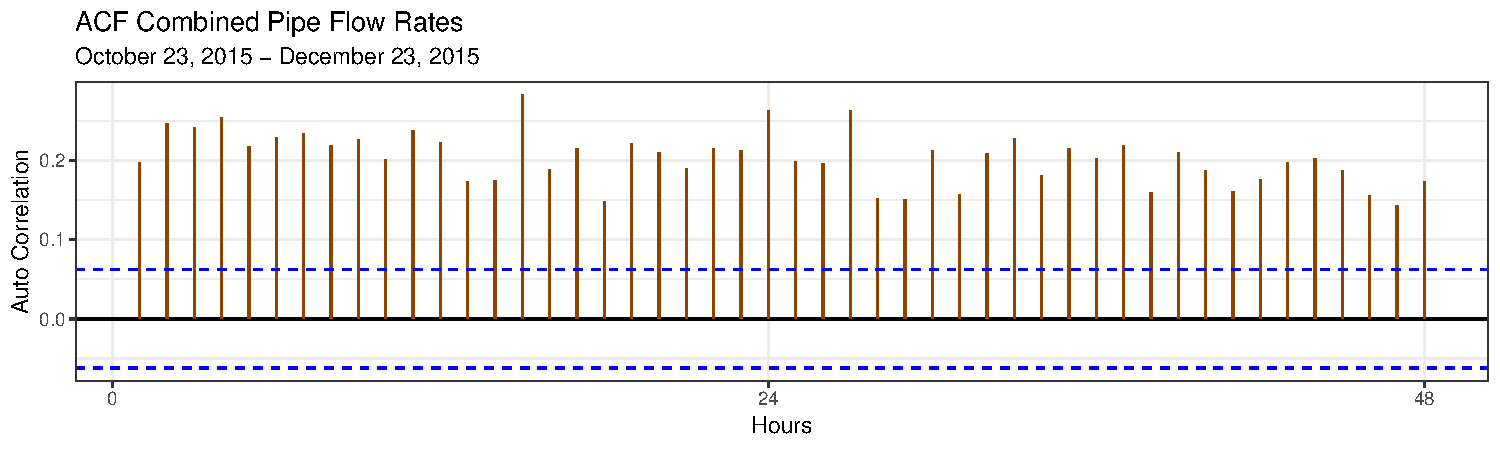
\includegraphics{Part-C-BP_files/figure-latex/unnamed-chunk-5-1.pdf}
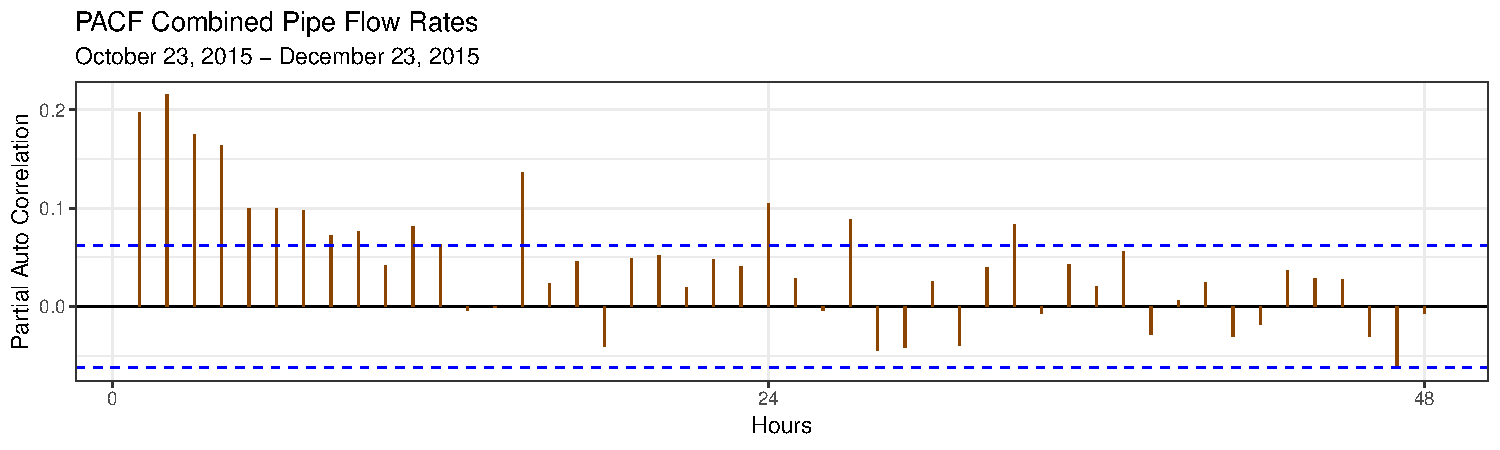
\includegraphics{Part-C-BP_files/figure-latex/unnamed-chunk-5-2.pdf}

\textbf{Interpreting the ACF and PACF}

The ACF remain wholly above the critical threshold, so will likely
require differencing as suggested by the \texttt{ndiffs()}, in looking
at the PACF, there is some abiguity caused by the needed differencing,
but after the intial trend down below the critical threshold, there is
definitely a slight spike at 24, which would suggest there may indeed by
a daily period or season we need to account for in our forecast.

\newpage

\textbf{Differenced ACF}

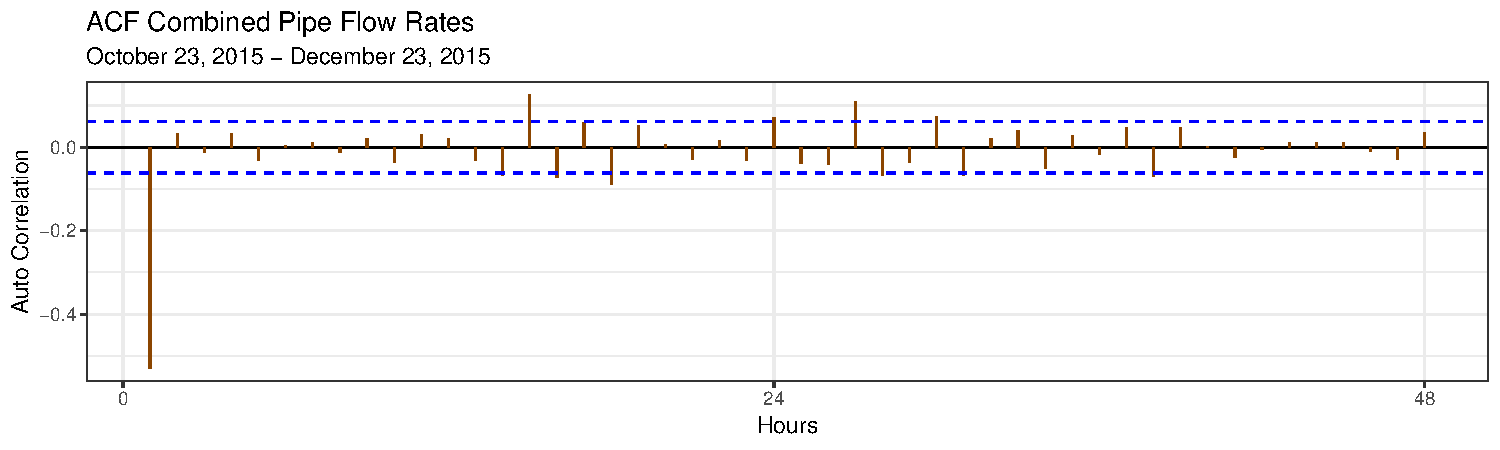
\includegraphics{Part-C-BP_files/figure-latex/unnamed-chunk-6-1.pdf}
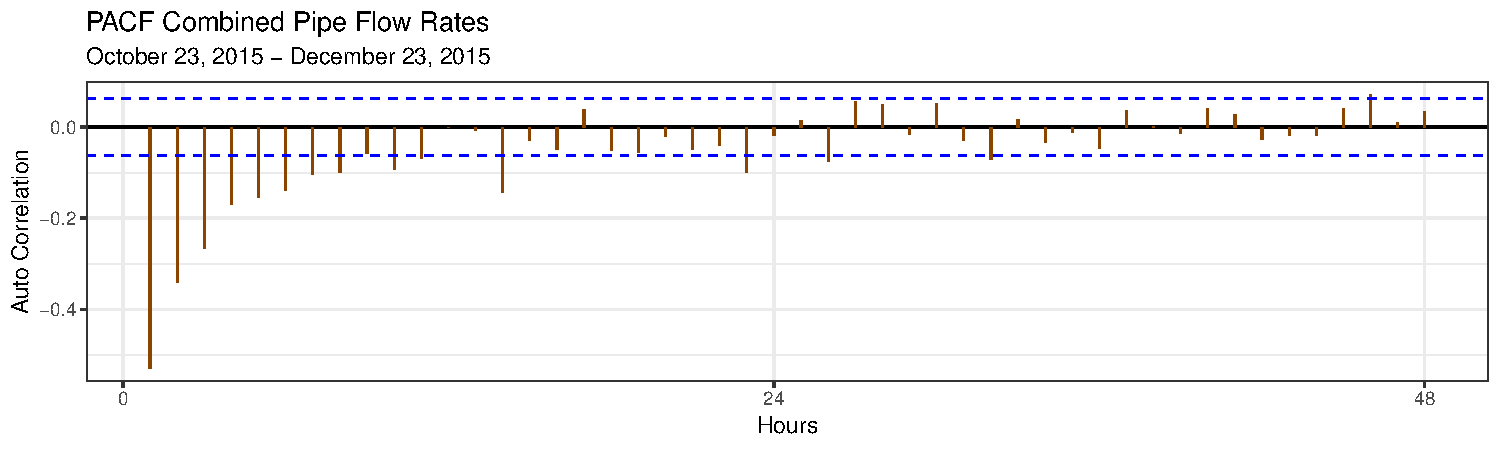
\includegraphics{Part-C-BP_files/figure-latex/unnamed-chunk-6-2.pdf}

A final ACF of the differenced data was done to ensure that a seconf
first-order difference was not needed; thus we assume \(d = 1\), a but
it was not so clear about the appropriate value of \$q4 should it be 5?
, so \texttt{auto.arima()} is in order to help iterate up on the likely
best starting place

\hypertarget{auto.arima}{%
\section{\texorpdfstring{\texttt{auto.arima()}}{auto.arima()}}\label{auto.arima}}

Using a Box-Cox lambda value to normalize the data may make
\(\lambda= .931552\). Because models can vary a lot based on the
selection criterion, both BIC and AIC models were run, using lambda, to
estimate a good starting place. We included the transformations in the
model (instead of doing it outside the model), because we are using the
ARIMA function to difference the data automatically allow more
constiency and flexibility in testing other model orders.

The \emph{AICc} chose a seasonal ARIMA of the following order:

\(ARIMA(1,1,3)(0,0,1)[24]\) \emph{AIC=7359.84 AICc=7359.9 BIC=7384.38}

The \emph{BIC} chose a non-seasonal ARIMA model as follows:

\(ARIMA(2,1,1)\) \emph{AIC=8082.22 AICc=8082.26 BIC=8101.85}

In both cases, the arima estimated that there needed to be differencing
which was supported by \texttt{ndiffs()} and our ACF \& PACF plots.

In comparing the two forecasts, for these automated models, they both
degrade toward the series mean pretty quickly, however, the AICc model
makes forecasts which consider the variation of the model a bit better
before it levels out. So we decided to explore this model and see if we
could tune it to provide more robust predictions

\textbf{AIC \(ARIMA(1,1,3)(0,0,1)[24]\) Residual Plots}

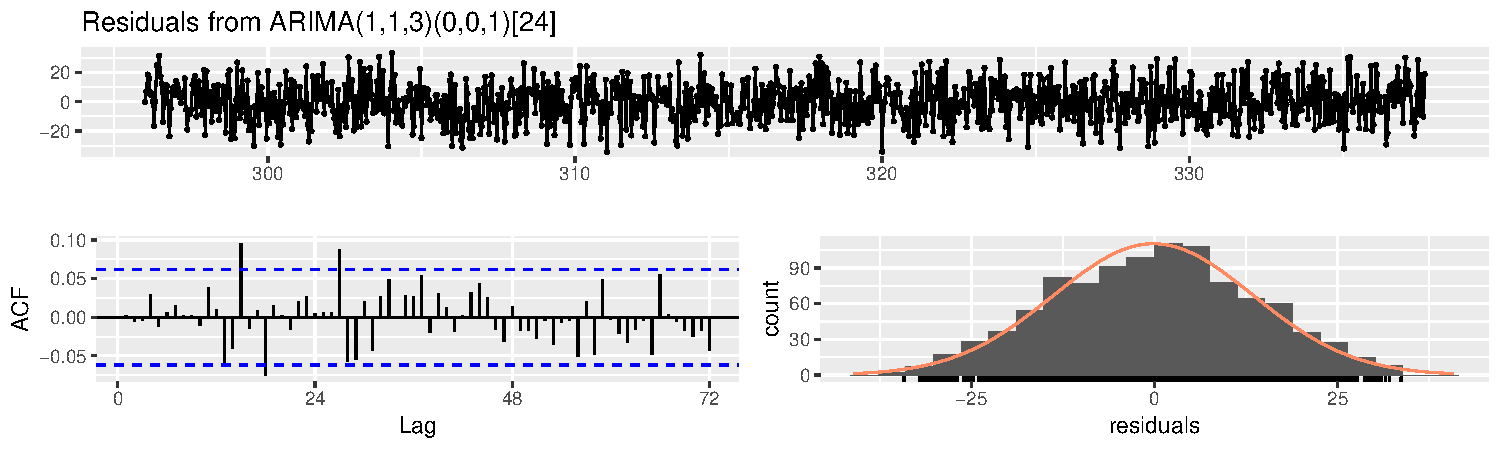
\includegraphics{Part-C-BP_files/figure-latex/unnamed-chunk-7-1.pdf}

\begin{verbatim}
FALSE 
FALSE   Ljung-Box test
FALSE 
FALSE data:  Residuals from ARIMA(1,1,3)(0,0,1)[24]
FALSE Q* = 57.362, df = 43, p-value = 0.07027
FALSE 
FALSE Model df: 5.   Total lags used: 48
\end{verbatim}

\textbf{BIC \(ARIMA(2,1,1)\) Residual Plots}

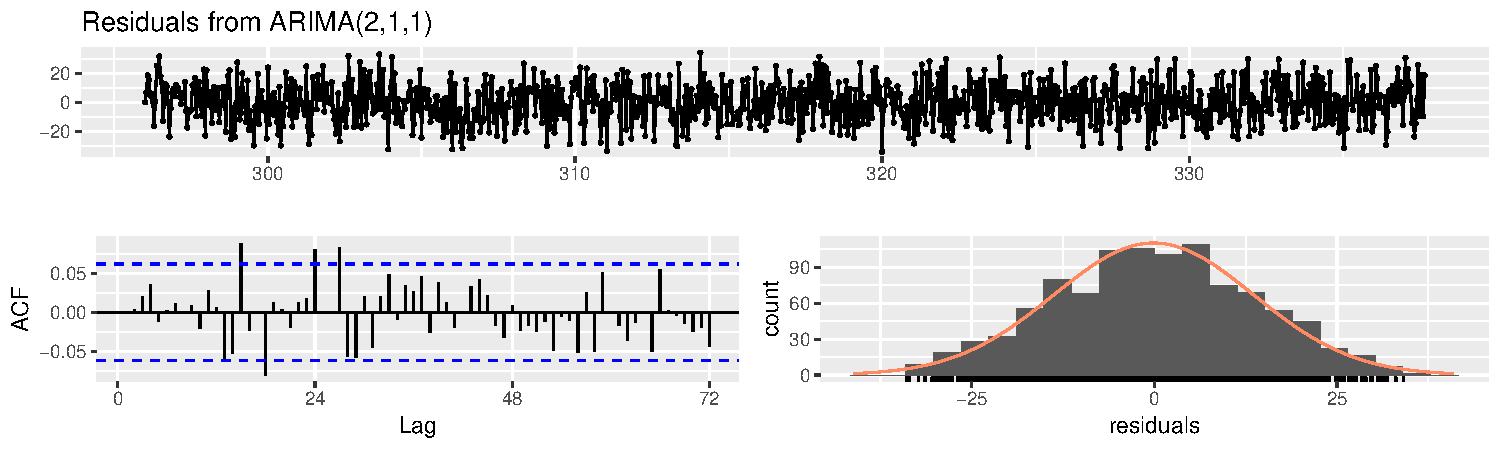
\includegraphics{Part-C-BP_files/figure-latex/unnamed-chunk-8-1.pdf}

\begin{verbatim}
FALSE 
FALSE   Ljung-Box test
FALSE 
FALSE data:  Residuals from ARIMA(2,1,1)
FALSE Q* = 64.403, df = 45, p-value = 0.03029
FALSE 
FALSE Model df: 3.   Total lags used: 48
\end{verbatim}

\hypertarget{interpreting-auto.arima}{%
\subsection{\texorpdfstring{Interpreting
\texttt{auto.arima()}}{Interpreting auto.arima()}}\label{interpreting-auto.arima}}

In looking at the AICc and BIC ARIMA models, the both appear to be
relatively white-noisy with no autocorrelation on the first or 24th
observations, with relatively normal residuals. However, in looking at
the Ljung-Box test for independence, it is clear that the Seasonal
\(ARIMA (1,1,3)(0,0,1)[24]\) is independent, where the \(ARIMA(2,1,1)\)
is not, thus reaffirming the lingering suspicion that thee is
unaccounted for seasonal variation in the model requiring a seasona
MA(1) to rectify. To be sure that the best model has been found, p \& q
as well as Q will be varied to see if a slight modification improves the
performance of the model.

\hypertarget{manual-arima-testing}{%
\subsection{Manual ARIMA testing}\label{manual-arima-testing}}

\begin{verbatim}
FALSE Series: ws 
FALSE ARIMA(1,1,3)(0,0,1)[24] 
FALSE Box Cox transformation: lambda= 0.9531552 
FALSE 
FALSE Coefficients:
FALSE          ar1      ma1     ma2      ma3    sma1
FALSE       0.7602  -1.7578  0.8286  -0.0614  0.0833
FALSE s.e.  0.1857   0.1874  0.1886   0.0324  0.0320
FALSE 
FALSE sigma^2 estimated as 187:  log likelihood=-4033.28
FALSE AIC=8078.56   AICc=8078.64   BIC=8108
\end{verbatim}

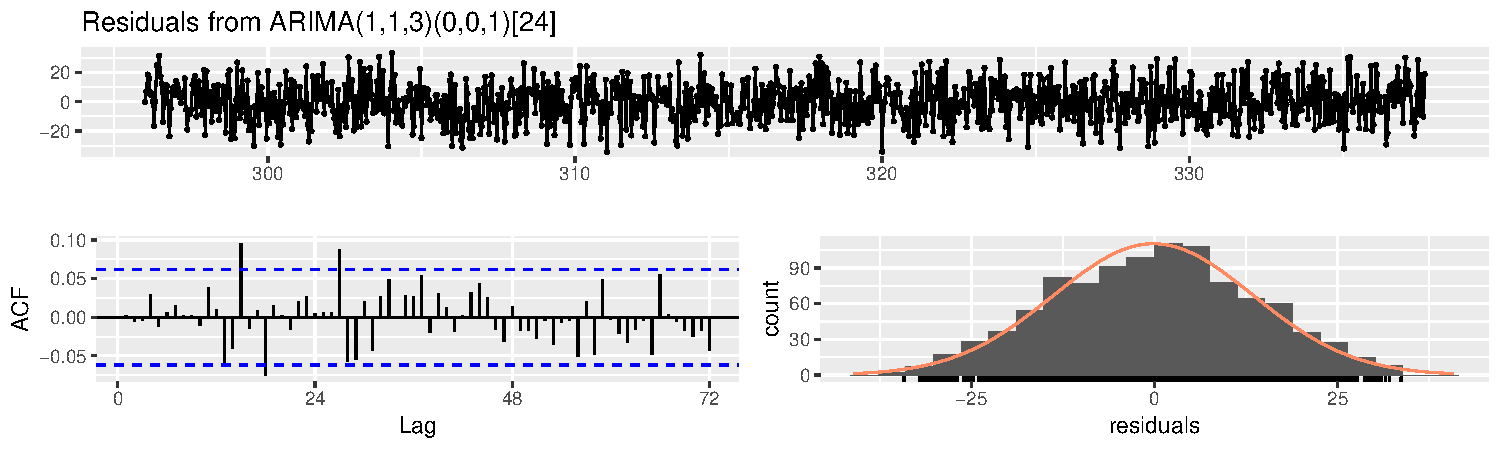
\includegraphics{Part-C-BP_files/figure-latex/unnamed-chunk-9-1.pdf}

\begin{verbatim}
FALSE 
FALSE   Ljung-Box test
FALSE 
FALSE data:  Residuals from ARIMA(1,1,3)(0,0,1)[24]
FALSE Q* = 47.142, df = 31, p-value = 0.03174
FALSE 
FALSE Model df: 5.   Total lags used: 36
\end{verbatim}

\hypertarget{forecasting-from-the-arima}{%
\subsubsection{Forecasting From the
ARIMA}\label{forecasting-from-the-arima}}

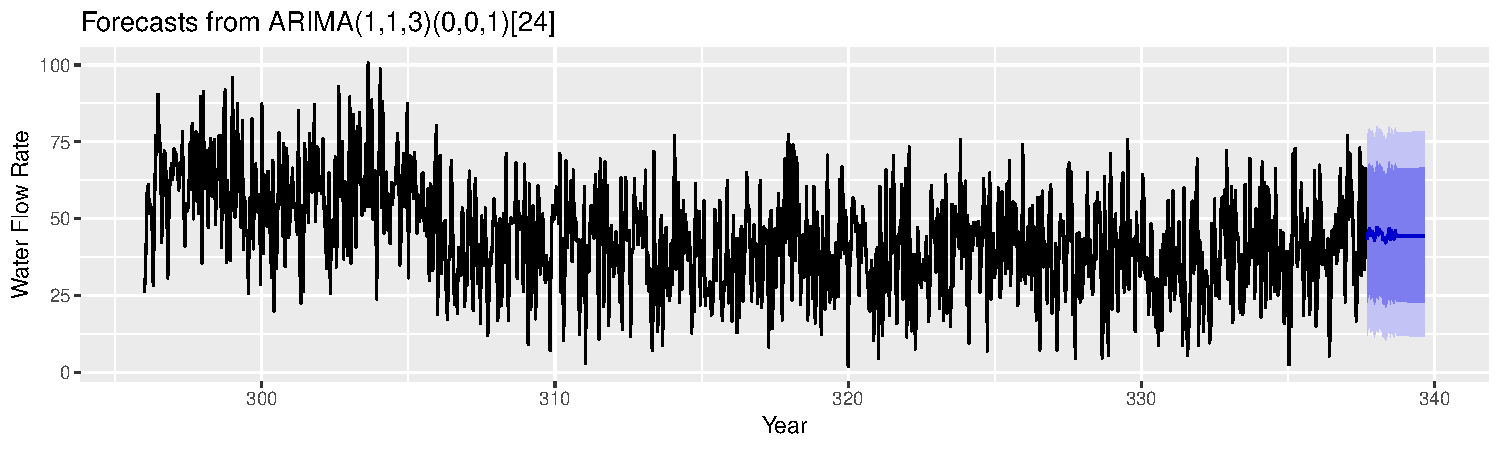
\includegraphics{Part-C-BP_files/figure-latex/unnamed-chunk-10-1.pdf}

\hypertarget{arima21300124}{%
\subsubsection{\texorpdfstring{\(ARIMA(2,1,3)(0,0,1)[24]\)}{ARIMA(2,1,3)(0,0,1){[}24{]}}}\label{arima21300124}}

\begin{verbatim}
FALSE Series: ws 
FALSE ARIMA(2,1,3)(0,0,1)[24] 
FALSE Box Cox transformation: lambda= 0.9531552 
FALSE 
FALSE Coefficients:
FALSE           ar1     ar2      ma1      ma2     ma3    sma1
FALSE       -0.1435  0.1884  -0.8478  -0.2709  0.1621  0.0798
FALSE s.e.      NaN  0.5408      NaN   0.6069  0.5320  0.0318
FALSE 
FALSE sigma^2 estimated as 187.5:  log likelihood=-4034.02
FALSE AIC=8082.05   AICc=8082.16   BIC=8116.4
\end{verbatim}

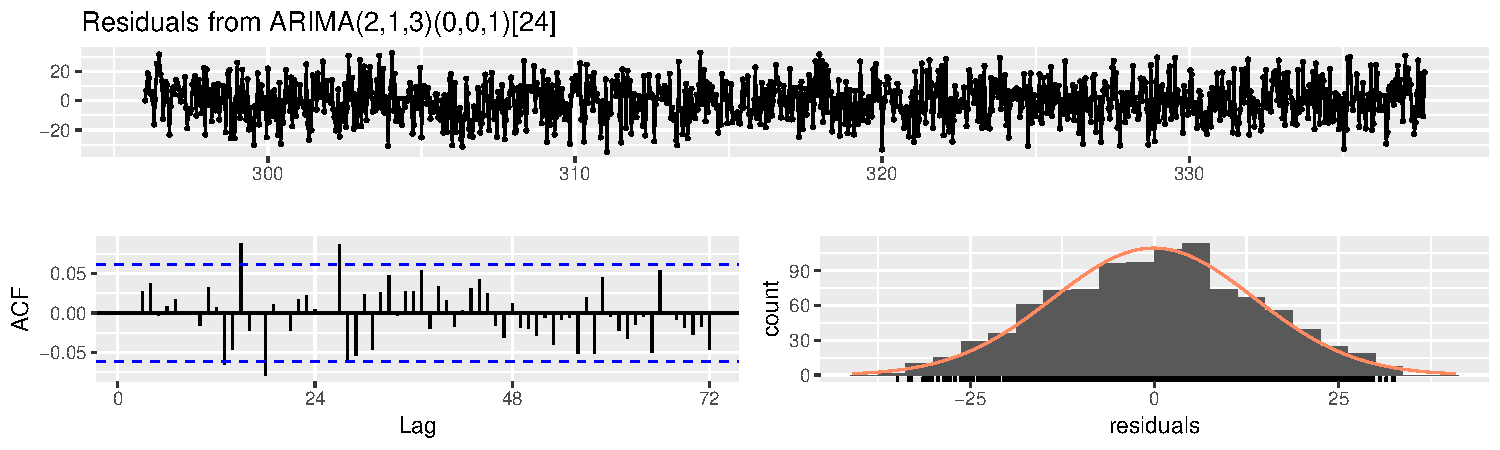
\includegraphics{Part-C-BP_files/figure-latex/unnamed-chunk-11-1.pdf}

\begin{verbatim}
FALSE 
FALSE   Ljung-Box test
FALSE 
FALSE data:  Residuals from ARIMA(2,1,3)(0,0,1)[24]
FALSE Q* = 48.506, df = 30, p-value = 0.01764
FALSE 
FALSE Model df: 6.   Total lags used: 36
\end{verbatim}

This Ljung-Box shows unexplained variances in the residuals indicating
that this model is not yet fully realized and inferior to the Seasonal
\(ARIMA (1,1,3)(0,0,1)[24]\).

\begin{verbatim}
FALSE Series: ws 
FALSE ARIMA(1,1,2)(0,0,1)[24] 
FALSE Box Cox transformation: lambda= 0.9531552 
FALSE 
FALSE Coefficients:
FALSE           ar1      ma1      ma2    sma1
FALSE       -0.2655  -0.7307  -0.2104  0.0790
FALSE s.e.   0.9490   0.9533   0.9121  0.0318
FALSE 
FALSE sigma^2 estimated as 187.1:  log likelihood=-4034.08
FALSE AIC=8078.16   AICc=8078.22   BIC=8102.7
\end{verbatim}

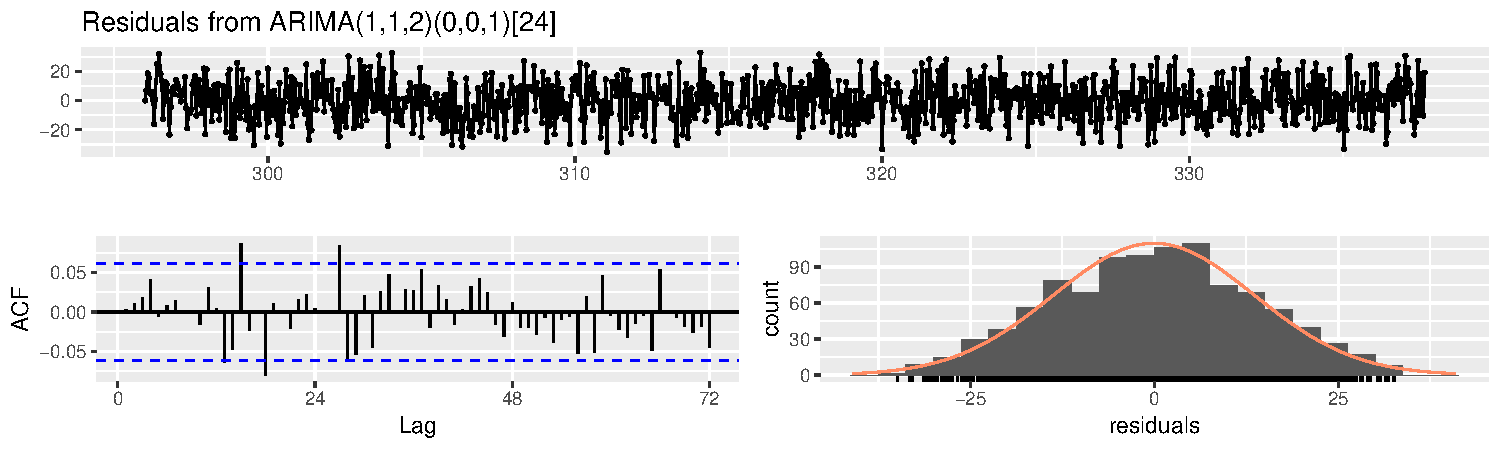
\includegraphics{Part-C-BP_files/figure-latex/unnamed-chunk-12-1.pdf}

\begin{verbatim}
FALSE 
FALSE   Ljung-Box test
FALSE 
FALSE data:  Residuals from ARIMA(1,1,2)(0,0,1)[24]
FALSE Q* = 47.963, df = 32, p-value = 0.03467
FALSE 
FALSE Model df: 4.   Total lags used: 36
\end{verbatim}

This Ljung-Box also shows unexplained variances in the residuals
indicating that this model is not yet fully realized and inferior to the
Seasonal \(ARIMA (1,1,2)(0,0,1)[24]\).

\begin{verbatim}
FALSE Series: ws 
FALSE ARIMA(1,1,3) 
FALSE Box Cox transformation: lambda= 0.9531552 
FALSE 
FALSE Coefficients:
FALSE          ar1      ma1     ma2      ma3
FALSE       0.6792  -1.6742  0.7437  -0.0553
FALSE s.e.  0.2923   0.2930  0.2903   0.0330
FALSE 
FALSE sigma^2 estimated as 188.1:  log likelihood=-4036.63
FALSE AIC=8083.27   AICc=8083.33   BIC=8107.81
\end{verbatim}

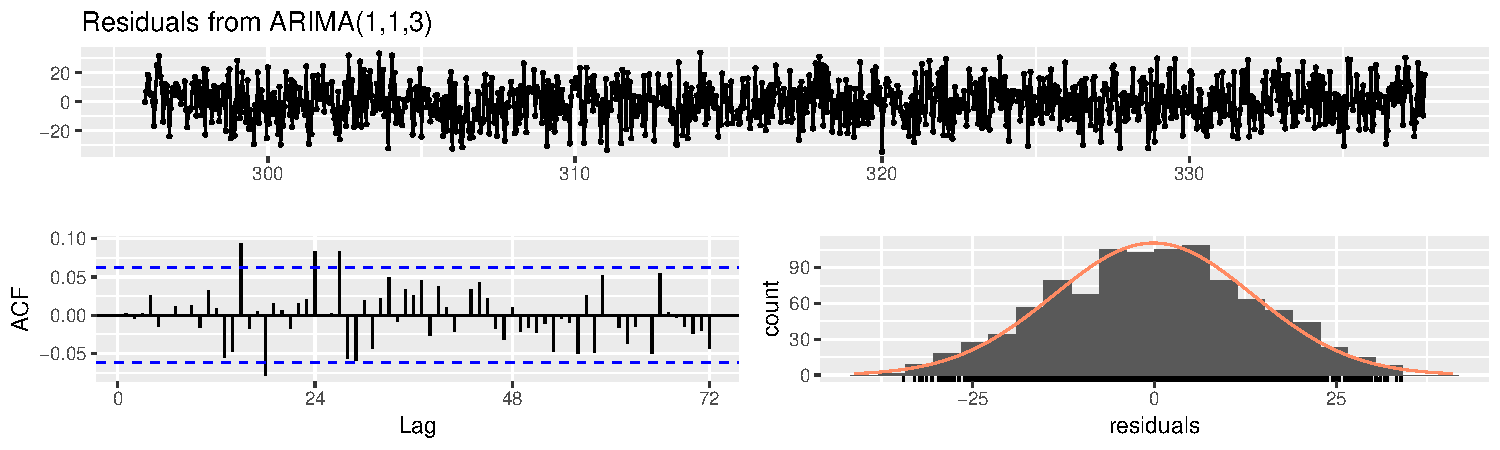
\includegraphics{Part-C-BP_files/figure-latex/unnamed-chunk-13-1.pdf}

\begin{verbatim}
FALSE 
FALSE   Ljung-Box test
FALSE 
FALSE data:  Residuals from ARIMA(1,1,3)
FALSE Q* = 53.61, df = 32, p-value = 0.009708
FALSE 
FALSE Model df: 4.   Total lags used: 36
\end{verbatim}

This Ljung-Box also shows unexplained variances in the residuals
indicating that this model is not yet fully realized and inferior to the
Seasonal \(ARIMA (1,1,3)\).

\hypertarget{accepting-the-auto.arima}{%
\subsection{\texorpdfstring{Accepting the
\texttt{auto.arima()}}{Accepting the auto.arima()}}\label{accepting-the-auto.arima}}

Given that the other models show unexplained variance in the residuals,
the final predictions will be made using the AICc recommended model of
\(ARIMA (1,1,3)(0,0,1)[24]\).

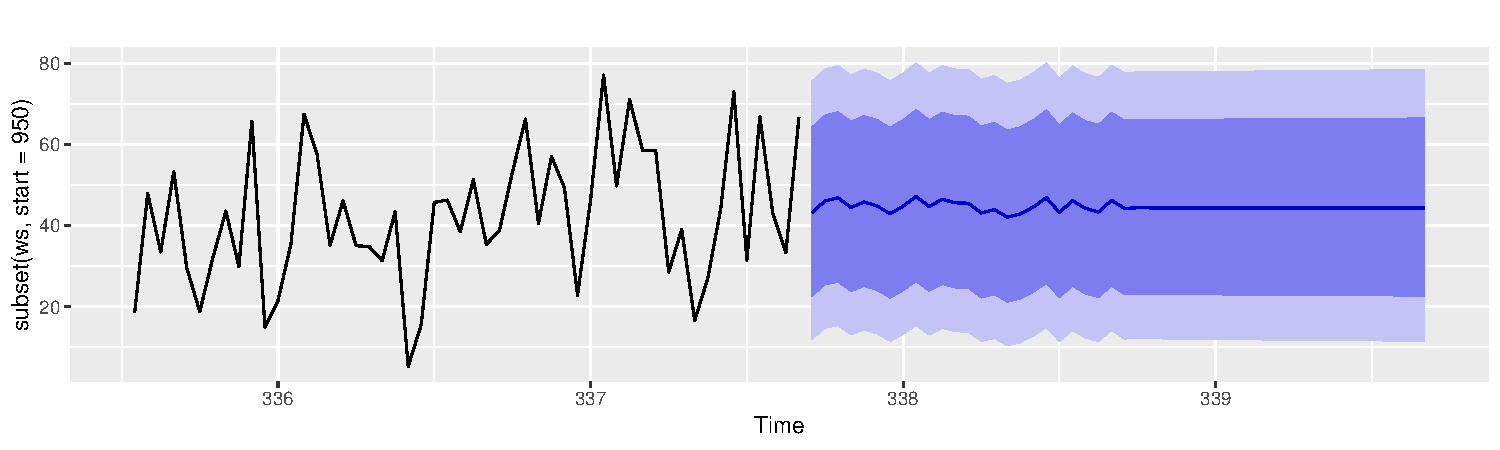
\includegraphics{Part-C-BP_files/figure-latex/unnamed-chunk-14-1.pdf}

\textbf{Sample Forecasts}

\begin{table}[t]

\caption{\label{tab:unnamed-chunk-15}First few predictions in the set}
\centering
\begin{tabular}{l|r|r|r|r|r}
\hline
DateTime & Point Forecast & Lo 80 & Hi 80 & Lo 95 & Hi 95\\
\hline
2015-12-03 17:00:00 & 43.21837 & 22.59441 & 64.33311 & 12.00034 & 75.65243\\
\hline
2015-12-03 18:00:00 & 46.07958 & 25.37341 & 67.24682 & 14.70394 & 78.58795\\
\hline
2015-12-03 19:00:00 & 46.85016 & 26.06919 & 68.08732 & 15.35468 & 79.46457\\
\hline
2015-12-03 20:00:00 & 44.49638 & 23.73897 & 65.73546 & 13.06315 & 77.11903\\
\hline
2015-12-03 21:00:00 & 45.83029 & 25.00018 & 67.13008 & 14.27275 & 78.54342\\
\hline
2015-12-03 22:00:00 & 44.85032 & 24.01864 & 66.16308 & 13.30217 & 77.58566\\
\hline
\end{tabular}
\end{table}

\hypertarget{forecast-accuracy}{%
\subsubsection{Forecast Accuracy}\label{forecast-accuracy}}

\begin{tabular}{l|r|r|r|r|r|r|r}
\hline
  & ME & RMSE & MAE & MPE & MAPE & MASE & ACF1\\
\hline
Training set & 0.0015679 & 16.27402 & 13.23093 & -28.76247 & 50.34448 & 0.7489308 & 0.0014339\\
\hline
\end{tabular}

\hypertarget{summary}{%
\section{Summary}\label{summary}}

Ultimately this model is marginally useful as seen by the Mean Absolute
Percentage of Error which reveals that the average percentage each
forecast is off by is around 50\%. In looking at the graph of the
forecast above, which is the last 150 points in the time series and the
forecasted points, you can see this as the predictions lightly modulate
around the mean and deteriorate to it pretty quickly.

In looking at the original decomposition, there very little trend, a lot
of seasonality, is a pretty substatial amount of random noise, which is
not considered in the model, and is responsible for the majority of the
error in this model, as white noise is never predictable.


\end{document}
